\documentclass{article}
\IfFileExists{iclr2025_conference.sty}{\usepackage{iclr2025_conference,times}}{
  \usepackage[margin=1in]{geometry}\usepackage{times}
  \usepackage[round,authoryear]{natbib}}
\usepackage[T1]{fontenc}
\usepackage[utf8]{inputenc}
\usepackage{amsmath,amssymb,booktabs,graphicx,microtype,xcolor,enumitem,multirow}
\usepackage{flafter}
\usepackage{tikz}
\usetikzlibrary{arrows.meta,positioning,fit}
\usepackage{hyperref,url}
\definecolor{dynblue}{HTML}{DCEBFA}
\definecolor{physorange}{HTML}{FBE4CB}
\definecolor{datagreen}{HTML}{DDEFD8}
\definecolor{learnpurple}{HTML}{E9DDF2}
\definecolor{projred}{HTML}{F5D4D4}
\newcommand{\model}{\textsc{DiffMars}}
\newcommand{\Ls}{L_\mathrm{s}}

\title{A Differentiable General Circulation Model for Mars}
\author{Anonymous authors}
% \iclrfinalcopy

\begin{document}
\maketitle

\begin{abstract}

General circulation models (GCMs) are the primary tool for simulating planetary atmospheres. They play a vital role in understanding Mars's atmosphere, as forecasting its unique weather is mission-critical for operations such as entry, descent, and landing. Mars poses unusual challenges for these models, as observations are sparse compared to Earth; a thin $CO_2$ atmosphere alongside a radiatively active dust cycle creates a volatile atmosphere with large diurnal temperature swings and no true terrestrial analog for validation. Existing Mars GCMs, including the LMD PCM, the NASA Ames Mars GCM, and PlanetWRF, are mature and physically detailed but are implemented with legacy Fortran using finite-difference or finite-volume solvers. Here we present a modular differentiable Mars GCM that couples Mars's unique atmospheric dynamics (radiative transfer, dust, $CO_2$ frost cycle, etc.) to the Dinosaur dynamical core. We showcase stable multi-Mars-year simulations that reproduce accurate seasonal evolution of the Martian atmosphere, capture realistic large-scale surface-temperature structure, and pressure correlated with MOLA elevation topology. We compare with conventional GCMs, highlighting the framework's computational efficiency and differentiability. We further outline extending the framework with a neural operator to represent unresolved processes while preserving Mars-specific physics.
\end{abstract}




\section{Introduction}

Mars is a useful and unusually strict test of hybrid climate modeling. Its thin,
mostly \(\mathrm{CO_2}\) atmosphere is coupled to large relief, strong seasonal
and diurnal forcing, and heterogeneous surface properties. In winter, a material
fraction of the atmosphere condenses onto the polar surface and returns in
spring \citep{leighton1966co2,guo2009seasonal}. Airborne dust both attenuates
sunlight and heats the atmosphere, changing thermal tides and the global
circulation \citep{madeleine2011dust,montabone2015dust}. Low atmospheric heat
capacity couples those effects tightly to regolith heat storage and boundary-layer
mixing. A model can therefore match one field for the wrong reason: excess
infrared opacity can offset weak soil storage, while excess drag can hide an
incorrect vertical heating profile.

The observing system makes such compensating errors difficult to identify.
MOLA and TES constrain topography and surface properties
\citep{smith2001mola,christensen2001tes}, while landers such as InSight provide
high-frequency local weather \citep{banfield2020insight}. There is no uniformly
observed global atmospheric state. Mars Climate Sounder profiles constrain
temperature, water vapor, dust, condensates, and polar energy balance
\citep{mccleese2007mcs}. MACDA, EMARS, and OpenMARS assimilate
spacecraft retrievals into different Mars GCMs
\citep{montabone2014macda,greybush2019emars,holmes2020openmars}. These products
are indispensable references, but they retain model and assimilation assumptions.

Mature physical Mars GCMs encode decades of knowledge. PlanetWRF spans local to
global planetary circulation \citep{richardson2007planetwrf}; the LMD planetary
climate model and NASA Ames GCM include vertically resolved radiation, dust, surface
thermodynamics, turbulent mixing, and volatile cycles
\citep{forget1999improved,haberle2019ames}. Their computational cost grows with
resolution, and resolution itself changes wave--mean-flow interactions
\citep{kling2025resolution}. A new model must consequently demonstrate more than
low snapshot error: it must show stability, closed budgets, seasonal phase and
amplitude, vertical structure, and measured computational cost.

NeuralGCM provides the architectural precedent. It combines a differentiable
spectral core with learned physical tendencies and trains the coupled model end
to end \citep{kochkov2024neuralgcm}. Stable learned closures require prognostic,
not merely one-step, validation \citep{yuval2020stable}. Fully differentiable
intermediate-complexity models likewise support parameter inference and coupled
optimization \citep{davenport2026jcm}. Recent Mars foundation models instead
learn fast global forecasts directly from reanalysis
\citep{roy2026foundation,singh2026aircast}. Our complementary goal is an
auditable physics-first simulator whose learned component is narrow, whose
reservoirs remain explicit, and whose errors can be traced to processes.

This distinction matters for planetary experiments. A hybrid GCM can expose
derivatives with respect to physical parameters or forcing, but only if those
derivatives pass through a stable, meaningful climate model. The longer-term
motivation includes controlled planetary-climate experiments. Although warming
proposals have a long history \citep{sagan1973planetary,mckay1991making},
accessible Martian \(\mathrm{CO_2}\) cannot produce an Earth-like climate
\citep{jakosky2018inventory}. Present-day validation is therefore a prerequisite;
recent calls for terraforming research do not remove that validation requirement
\citep{debenedictis2025case}. This paper makes no terraforming-outcome claim.

Our central question is narrower: can a compact differentiable Mars GCM
survive a complete seasonal cycle while preserving the dominant mass budget and
exposing identifiable physical errors? We answer with a hierarchy of evidence.
Core tests establish implementation correctness; a complete Mars-year rollout
tests stability and conservation; MOLA, ARCO-MACDA, Ames, and MCD provide
complementary structural and climatic diagnostics; and measured throughput
establishes the cost of producing those results.

Our contributions are: (i) a planet-parameterized Mars GCM built on the
Dinosaur core used by NeuralGCM \citep{dinosaur2024}; (ii) explicit orbit,
multiband radiation, dust, surface, regolith, boundary-layer, convection, and
seasonal-cap operators connected by a typed tendency interface; (iii) an
atmosphere--surface \(\mathrm{CO_2}\) projection and scale-selective diffusion
that permit a clean 668-sol integration; (iv) a versioned ARCO-MACDA pipeline
with a leakage-safe Mars-year split; and (v) executable evidence for gradients,
mass conservation, topographic structure, reference error, failure diagnosis,
and runtime. The resulting evidence defines both the model's current capability
and the physical errors that must be resolved before learned closure training.

\section{Background and Related Work}

\subsection{Mars models and reference products}
PlanetWRF provides a general local-to-global dynamical framework
\citep{richardson2007planetwrf}. The LMD model established a comprehensive
framework extending above 80 km \citep{forget1999improved}; NASA Ames supplies
an independently developed reference \citep{haberle2019ames}. MCD v6.1 exposes LMD simulations through
season-, location-, altitude-, local-time-, and dust-matched queries
\citep{mcd61}. We treat Ames and MCD as model references, never observational
truth. MOLA and TES are static boundary inputs. MACDA, EMARS, and OpenMARS are
data-assimilating products, and comparing them reveals sensitivity to the parent
model and assimilation system. ARCO-Mars republishes all three as cloud-optimized
archives, allowing bounded reads instead of full downloads
\citep{bhattacharya2026arcomars}.

The reference roles are intentionally separate. ARCO-MACDA supplies consecutive
global states for diagnostics and possible closure training; ARCO-EMARS and
ARCO-OpenMARS can quantify reference dependence. Ames and MCD provide
model-family comparisons, while lander records provide direct observational
anchors. No product serves simultaneously as a boundary condition and sole
evaluation target.

\subsection{Coupled Mars processes}
Orbital geometry and surface properties set solar heating; regolith storage and
turbulent exchange determine its diurnal and seasonal response. Dust adds solar
scattering and absorption as well as infrared opacity
\citep{madeleine2011dust}. Because gaseous absorption varies with wavelength,
pressure, and temperature, two-stream and correlated-\(k\) methods compress a
costly spectral transfer problem \citep{toon1989twostream}. The vertical heating
profile matters as much as the surface mean because winds respond to horizontal
and vertical temperature gradients. At the polar caps, condensation couples
latent heat, surface optics, atmospheric mass, and circulation. These links
motivate explicit process operators and budget tests before residual learning.

\subsection{Differentiable climate models}
NeuralGCM combines spectral primitive-equation dynamics with learned
parameterizations \citep{kochkov2024neuralgcm}; JCM shows that an
intermediate-complexity atmosphere can be fully differentiable
\citep{davenport2026jcm}. \model{} follows their resolved-dynamics/column-physics
split while first establishing deterministic Mars operators, explicit
reservoirs, and long-rollout diagnostics. This physics-first ordering prevents
a learned tendency from concealing defects in mass conservation, radiation, or
surface exchange.

\subsection{Verification before learning}
A residual can hide a numerical defect while reducing loss. We therefore use
standard spherical and atmospheric-core tests
\citep{williamson1992standard,held1994proposal,jablonowski2006baroclinic}, then
measure column-energy closure, surface exchange, frost positivity, total
\(\mathrm{CO_2}\), topographic pressure, and seasonal stability.

We measure numerical correctness, volatile conservation, season- and
local-time-matched climatic fidelity, and computational cost. Each diagnostic
has a distinct interpretation: structural agreement is not treated as forecast
skill, and a model-product comparison is not treated as observational truth.

\section{Method}

\subsection{Coupled formulation}
Let \(x_t\) contain spectral vorticity, divergence, temperature variation,
log-surface-pressure, and time, and let \(s_t\) contain surface temperature,
\(\mathrm{CO_2}\)-ice pressure equivalent, and soil temperatures:
\begin{equation}
\frac{d}{dt}\begin{bmatrix}x\\s\end{bmatrix}
=\mathcal D(x;b)+\mathcal P(x,s,b,t).
\label{eq:hybrid}
\end{equation}
\(\mathcal D\) is resolved dynamics, \(\mathcal P\) is deterministic column
physics, and \(b\) contains fixed boundary fields.

\begin{figure}[t]
\centering
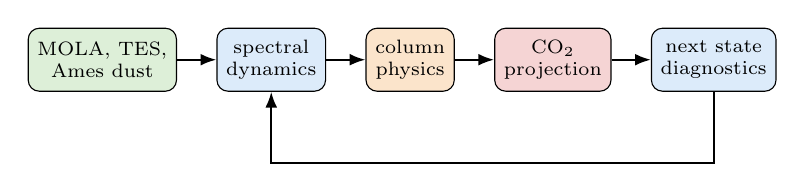
\begin{tikzpicture}[node distance=4mm and 5mm,
 box/.style={draw,rounded corners,align=center,minimum height=8mm,font=\scriptsize},
 arr/.style={-{Latex[length=2mm]},thick}]
\node[box,fill=datagreen] (data) {MOLA, TES,\\Ames dust};
\node[box,fill=dynblue,right=of data] (dyn) {spectral\\dynamics};
\node[box,fill=physorange,right=of dyn] (phys) {column\\physics};
\node[box,fill=projred,right=of phys] (proj) {CO\(_2\)\\projection};
\node[box,fill=dynblue,right=of proj] (out) {next state\\diagnostics};
\draw[arr] (data)--(dyn);\draw[arr] (dyn)--(phys);\draw[arr] (phys)--(proj);
\draw[arr] (proj)--(out);
\draw[arr] (out.south)|-++(0,-9mm)-|(dyn.south);
\end{tikzpicture}
\caption{One \model{} step. Spectral dynamics and nodal column physics share a
typed state; the projection enforces the atmosphere--surface CO$_2$ inventory.}
\label{fig:architecture}
\end{figure}

\subsection{Software framework and execution path}
The implementation separates reusable numerics from Mars configuration. The
\texttt{framework/gcm} package defines coordinates, nondimensionalization,
Dinosaur adapters, IMEX integration, restarts, and benchmarks. The framework
physics module contains JAX-pure column operators and their typed tendency
contract. The Mars package owns
planetary constants, orbit, MOLA/TES staging, Ames dust, and run assembly.
Scripts add chunked execution, checkpoint diagnostics, reference staging, and
evaluation. This dependency direction prevents generic physics from silently
importing Mars constants.

Each physics evaluation transforms spectral fields once to nodal temperature,
wind, and pressure, then shares those arrays among radiation, surface exchange,
drag, PBL diffusion, convection, regolith conduction, and \(\mathrm{CO_2}\)
exchange. Radiation uses fixed-size \texttt{lax.scan} recurrences; vertical
diffusion uses a batched tridiagonal Thomas solve; and convection uses a
fixed-shape weighted pool-adjacent-violators scan. These choices keep compiled
timesteps free of data-dependent Python control flow and make the major column
kernels scale linearly with layer count.

\begin{table}[t]\centering\small
\caption{Implemented software layers.}\label{tab:framework}
\begin{tabular}{p{0.25\linewidth}p{0.67\linewidth}}\toprule
Layer & Responsibility\\\midrule
Dinosaur adapter & Spectral transforms, sigma coordinates, primitive equations,
IMEX step, hyperdiffusion\\
Column physics & Radiation, fluxes, drag, PBL, convection, soil, volatile cycle\\
Mars assembly & Constants, orbit, MOLA/TES, dust, balanced initialization\\
Run/evaluation & JIT rollout, restart, budgets, NetCDF, ARCO/Ames/MCD matching\\\bottomrule
\end{tabular}
\end{table}

\subsection{Resolved dynamics and numerical integration}
The Dinosaur/JAX core \citep{dinosaur2024,jax2018} solves the hydrostatic
primitive equations in terrain-following \(\sigma=p/p_s\) coordinates. In
schematic vector form,
\begin{align}
\frac{D\mathbf v}{Dt}+f\mathbf k\!\times\!\mathbf v
 &= -\nabla_\sigma\Phi-RT\nabla_\sigma\log p_s+\mathbf F_{\rm phys},\\
\frac{DT}{Dt}-\kappa T\frac{D\log p}{Dt}&=Q_{\rm phys},\\
\frac{\partial\log p_s}{\partial t}
 &= -\frac{1}{p_s}\nabla\!\cdot\int_0^1p_s\mathbf v\,d\sigma+S_{\rm CO_2}.
\end{align}
Hydrostatic geopotential follows from \(\partial\Phi/\partial\log p=-RT\).
Vorticity and divergence avoid polar vector singularities. The core resolves
transport, pressure gradients, rotation, and gravity waves; column physics
supplies momentum, heat, and volatile sources.

Production uses T21 (a \(32\times64\) Gaussian nodal grid), 12 sigma layers, a
300\,s semi-implicit timestep, and fourth-order spectral diffusion with a
0.1-sol shortest-mode e-folding time. Diffusion acts only on modal atmospheric
fields, leaving nodal surface, frost, and soil reservoirs unchanged.

\subsection{Orbit, radiation, and dust}
Kepler's equation determines heliocentric distance, true anomaly, \(\Ls\), and
declination. Rotation and longitude determine local hour angle. The corrected
configuration resolves the diurnal zenith angle and slant optical path; the
completed baseline used daily-mean sunlight and is labeled accordingly.

Radiation uses seven solar and five thermal Ames bands, with 16 absorbing
correlated-\(k\) channels and one clear channel per band. Coefficients are
interpolated in temperature and log pressure. A two-stream recurrence propagates
upward and downward fluxes \citep{toon1989twostream}. Prescribed visible and
infrared dust opacity is distributed vertically with an Ames/Conrath profile and
band-dependent scattering and absorption. It represents the leading radiative
effect of dust but not lifting, transport, settling, or particle evolution
\citep{madeleine2011dust}.

Layer heating follows discrete net-flux convergence, so internal interface
fluxes cancel in the column energy budget.

\subsection{Surface, regolith, PBL, and convection}
Prognostic surface temperature obeys
\begin{equation}
C_s\frac{dT_s}{dt}=F^\downarrow_{\rm SW}-F^\uparrow_{\rm SW}
+F^\downarrow_{\rm LW}-\epsilon\sigma T_s^4-H-G-L_{\rm CO_2}\dot m,
\end{equation}
where \(H\) transfers sensible heat to the atmosphere, \(G\) enters the soil,
and \(\dot m\) is positive for condensation. TES supplies spatial albedo and
thermal inertia. Twelve finite-volume soil layers extend from fractions of the
diurnal skin depth to beyond the annual skin depth; internal conductive fluxes
cancel pairwise and soil state is checkpointed.

Log-law surface stress and sensible exchange are modified by bulk Richardson
stability. An implicit tridiagonal solve mixes heat, momentum, and tracers in the
PBL while conserving the appropriate column integral. Dry adjustment identifies
contiguous unstable blocks and conserves sigma-mass-weighted enthalpy. These
closures capture minimum constraints but remain simpler than mature plume and
Mellor--Yamada-style Mars schemes
\citep{forget1999improved,haberle2019ames,colaitis2013pbl}.

\subsection{Seasonal \texorpdfstring{\(\mathrm{CO_2}\)}{CO2} cycle}
Surface \(\mathrm{CO_2}\) condenses or sublimes from the non-latent energy
residual at a pressure-dependent frost point. Supply and ice gates prevent
removing unavailable mass, and latent heat returns to the surface budget.
Atmospheric condensation, frost-dependent optics, and \(\mathrm{CO_2}\) clouds
remain absent.

Because the dycore advances \(\log p_s\), a finite step does not exactly preserve
the linear inventory conserved by the tendency. After each step, negative frost
is repaired and a global pressure scale \(\alpha\) satisfies
\begin{equation}
\int_A(\alpha p_s^*+p_{\rm ice}^*)\,dA
=\int_A(p_s+p_{\rm ice})\,dA-\Delta M_{\rm escape}g.
\end{equation}
Gaussian quadrature evaluates the integrals. The projection preserves the
resolved pressure pattern, maintains positive pressure, and retains an explicit
escape sink when configured.

\subsection{Reference data and metrics}
MOLA and TES are boundary inputs rather than evaluation targets. For the
reported diagnostic, we stream the season-matched MY24 ARCO-MACDA daily mean,
interpolate its 35 sigma levels to the model levels, regrid it to T21, and
record source provenance and hashes. Metrics use Gaussian spherical-area
weights. Relative MAE divides weighted absolute error by the weighted mean
absolute reference magnitude, avoiding the singular normalization produced by
near-zero signed global wind means. Comparisons record the mismatch in \(\Ls\),
averaging window, local time, vertical coordinate, and dust scenario. We label
MACDA and Ames results as model-reference diagnostics rather than observations.

\begin{table}[t]
\centering\small
\caption{Completed physical-baseline configuration.}\label{tab:config}
\begin{tabular}{ll}\toprule
Component & Choice\\\midrule
Grid/time & T21, \(32\times64\), 12 sigma levels, 300\,s\\
Boundary & MOLA; TES albedo and thermal inertia\\
Forcing & eccentric orbit; daily mean in completed run\\
Radiation & Ames correlated-\(k\) CO\(_2\); prescribed dust\\
Surface & prognostic skin, 12 soil layers, CO\(_2\) frost\\
Mixing & Richardson exchange, implicit PBL, dry adjustment\\
Dissipation & fourth order; 0.1-sol shortest-wave time\\\bottomrule
\end{tabular}
\end{table}

\section{Results}

\subsection{Verification and differentiability}
The focused GCM suite passed 127 tests with three skipped, including slow
core benchmarks; the full non-slow package suite passed 292 with three skipped
and five deselected long tests. These verify numerical and software contracts,
not climate accuracy.

For a T21/four-level eight-step rollout, the derivative of area-mean surface
temperature with respect to uniform albedo is \(-1.0341944645\) K per unit
albedo. Centered finite differences at \(10^{-3}\) and \(10^{-4}\) agree to
relative errors \(6.1\times10^{-10}\) and \(3.5\times10^{-9}\). This establishes
local differentiation through a smooth path, not useful seasonal gradients
across physical switches.

\begin{table}[t]\centering\small
\caption{Numerical evidence at this manuscript snapshot.}\label{tab:num}
\begin{tabular}{lll}\toprule
Check & Result & Scope\\\midrule
Autodiff vs finite difference & \(6.1\times10^{-10}\) & short smooth path\\
Completed integration & 668.0004 sols & finite first year\\
Maximum CO\(_2\) relative drift & \(1.22\times10^{-9}\) & projection effective\\
Pressure--elevation correlation & \(-0.960459\) & topographic structure\\
Final maximum 3-D wind & 129.729 m\,s\(^{-1}\) & finite upper level\\\bottomrule
\end{tabular}
\end{table}

\subsection{Failure diagnosis and stable baseline}
The first unfiltered attempt remained finite through sol 512.166 but reached
2953 m\,s\(^{-1}\) winds and then failed. Total \(\mathrm{CO_2}\) remained
conserved, separating the failure from volatile exchange. Fourth-order diffusion
reduced maximum wind to 46.0 m\,s\(^{-1}\) within 3.332 sols from the degraded
restart. We rejected that recovery and reran from initialization.

The clean run completed 197,673 steps (668.0004 sols); all exported values and
135 checkpoints are finite. Final surface pressure spans 221.82--1078.76 Pa,
temperature 144.33--241.22 K, and near-surface wind 0.20--30.02 m\,s\(^{-1}\).
Atmosphere-plus-frost \(\mathrm{CO_2}\) changed from
\(2.5984358236\times10^{16}\) to \(2.5984358204\times10^{16}\) kg, a relative
drift of \(-1.22\times10^{-9}\). This establishes numerical stability for one
Mars year, not equilibrium.

\subsection{Topography and ARCO-MACDA diagnostic}
T21 MOLA elevation ranges from \(-7.261\) to 14.478 km. Final pressure correlates
with elevation at \(-0.960459\), with a fitted 10.95 km log-pressure scale
height. This confirms boundary alignment and hydrostatic structure but is not an
independent target because MOLA initializes the lower boundary. We compare the
instantaneous state at \(\Ls=359.683^\circ\) to the MY24
ARCO daily mean at \(0.278^\circ\), a \(0.595^\circ\) offset. Pressure and broad
temperature structure agree; winds do not (Table~\ref{tab:arco}). The model is
13.40 K too warm, vector-wind correlations are 0.36--0.47, and frost relative
MAE is 42.9\%. Temporal mismatch and reanalysis ancestry make this diagnostic
rather than held-out validation.

\begin{table}[t]\centering\small
\caption{Area-weighted model--ARCO diagnostic. ARCO-MACDA is a reanalysis
reference rather than direct observational truth.}\label{tab:arco}
\begin{tabular}{lrrr}\toprule
Field & Bias & MAE & Corr.\\\midrule
Pressure (Pa) & \(-14.12\)&23.57&0.987\\
Surface \(T\) (K) & \(+13.40\)&13.40&0.953\\
East wind (m\,s\(^{-1}\)) & \(-1.16\)&5.48&0.469\\
North wind (m\,s\(^{-1}\)) & \(-1.38\)&5.46&0.361\\
Wind speed (m\,s\(^{-1}\)) & \(+3.45\)&4.71&0.455\\
CO\(_2\) frost (Pa-eq.) & \(-47.33\)&54.74&0.888\\\bottomrule
\end{tabular}
\end{table}

\begin{figure}[t]\centering
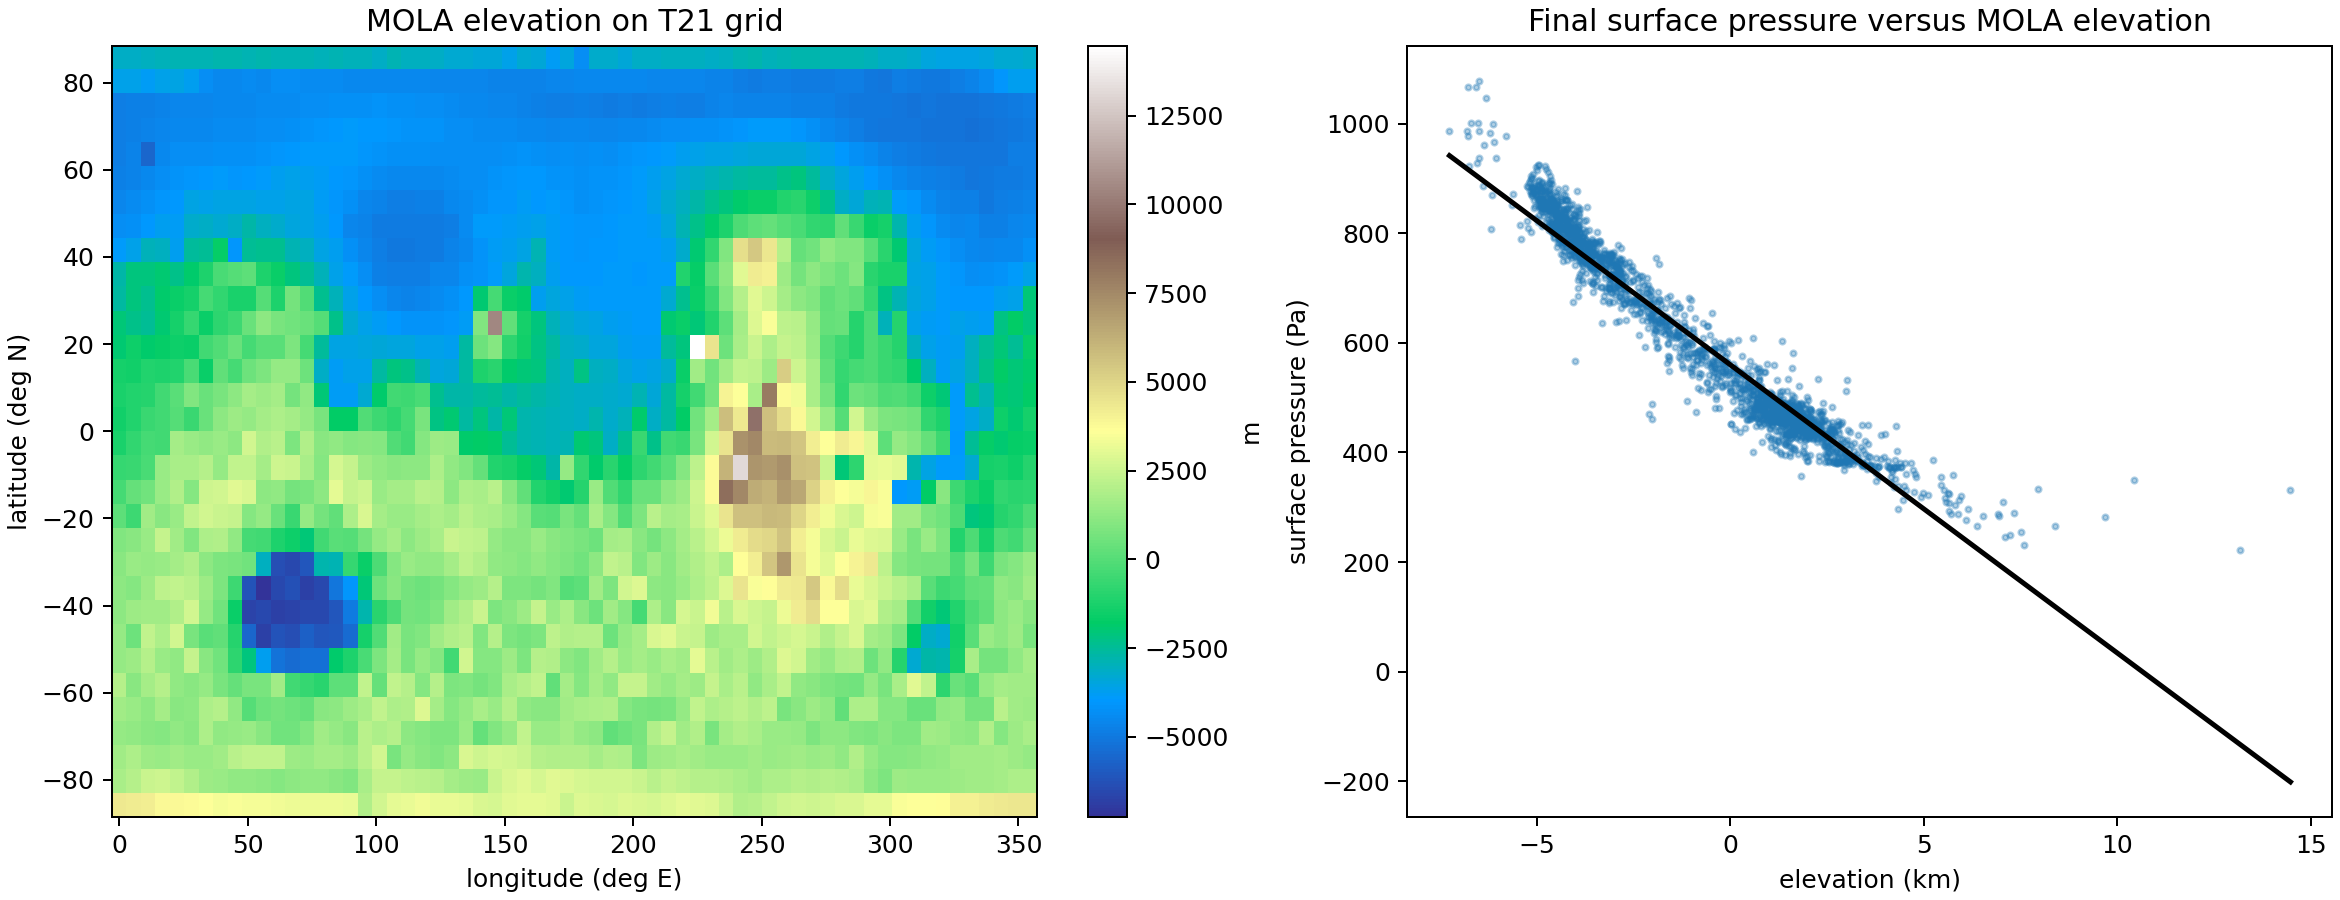
\includegraphics[width=\linewidth]{figures/mola_topography_pressure.png}
\caption{MOLA topography and final pressure versus elevation. This tests
boundary alignment and hydrostatic structure, not forecast skill.}\label{fig:mola}
\end{figure}

\subsection{Radiative-bias probes and corrected run}
The \(+13.4\) K bias motivated a process-level energy diagnosis. Daily-mean
sunlight suppresses the large Martian day--night cycle; because emission scales
as \(T^4\), that changes the mean energy balance. The original correlated-\(k\)
path also omitted the zenith-angle air-mass factor and did not use the separately
prescribed infrared dust field. These are identifiable physics-path errors.
Enabling resolved local time, slant paths, and
infrared dust in a ten-sol probe from the year-one restart
reduced matched Ames temperature bias to \(+6.93\) K (MAE 7.05 K, correlation
0.9716). Scaling CO\(_2\) and dust longwave opacity to 0.25 reduced bias to
\(+4.28\) K and MAE to 4.71 K, retaining 0.9720 correlation; its fixed-state TOA
imbalance was \(+0.433\) W\,m\(^{-2}\). These remain short diagnostics.

The exact two-orbital-period corrected run subsequently completed step 593,385
at sol 2005.2381 with finite fields. Its maximum relative combined
atmosphere--frost \(\mathrm{CO_2}\) drift was \(1.81\times10^{-9}\). Across
\(\Ls=45,135,225,315^\circ\), year-over-year changes passed the declared
thresholds for global mean pressure (maximum 2.50 Pa), frost (2.50 Pa), and
surface temperature (0.620 K). The overall convergence gate failed because deep
soil temperature changed by 0.442--0.634 K, above the 0.25 K threshold in every
season. The atmosphere and surface cycle are repeatable by these global metrics,
but the regolith is not yet equilibrated; seasonal Ames evaluation therefore
remains withheld.

\begin{table}[t]\centering\small
\caption{Maximum consecutive-year change over
$\Ls=45,135,225,315^\circ$ in the corrected run.}\label{tab:convergence}
\begin{tabular}{lrrl}\toprule
Quantity & Change & Threshold & Result\\\midrule
Mean surface pressure & 2.497 Pa & 5 Pa & pass\\
Mean CO$_2$ frost & 2.497 Pa-eq. & 5 Pa & pass\\
Mean surface temperature & 0.620 K & 1 K & pass\\
Deep-soil temperature & 0.634 K & 0.25 K & fail\\\bottomrule
\end{tabular}
\end{table}

\subsection{Measured computational cost}
The completed manifest records 190,273 post-restart steps in 21,453.3 s on an
11-core Apple M3 Pro with 18 GB memory. This is 8.88 steps s\(^{-1}\), 107.9
simulated sols per wall hour, or approximately 6.19 wall hours per 668-sol Mars
year after compilation. The timing excludes 7,400 steps completed by an earlier
invocation and is therefore steady-state throughput rather than end-to-end time.
Checkpoint cooldown and output settings also affect the value.

We do not claim a speedup over Ames, LMD, or NeuralGCM because their configurations
differ in hardware, resolution, physics, and output cadence. A fair final table
would require matched hardware, resolution, physics, and output cadence.

\section{Limitations}
\model{} is a coarse, dry present-day Mars model. It omits water, clouds,
atmospheric \(\mathrm{CO_2}\) condensation, interactive dust lifting and
sedimentation, frost-dependent optics, subgrid orographic drag, photochemistry,
and resolved upper-atmosphere escape. Prescribed dust cannot respond to simulated
winds. Radiation closes its discrete energy budget but still needs direct
Ames-column flux regression; the PBL and convection are simpler than mature
Mars closures.

One completed Mars year demonstrates finite integration, not equilibrium. It
uses daily-mean sunlight, while ARCO is a daily mean produced by a reanalysis.
The MY24 sample verifies the evaluation pipeline rather than generalization.
Ames and MACDA are model products. MOLA pressure structure is
not independent because topography is a boundary condition. Runtime is one
laptop measurement and excludes initial JIT compilation.

Differentiability is local: frost repair, stability transitions, and convective
block changes can create nonsmooth boundaries. A short finite gradient does not
guarantee an informative seasonal derivative. No trained residual, multi-seed
score, corrected equilibrium, held-out result, or intervention is reported.

\section{Conclusion}
We present a NeuralGCM-style foundation for Mars: differentiable spectral
dynamics, explicit orbital and column physics, conservative surface
\(\mathrm{CO_2}\), versioned data interfaces, and seasonal evaluation. Current
evidence supports a precise claim. \model{} differentiates through a short
coupled rollout, remains finite for a complete baseline year, limits volatile
drift to \(1.22\times10^{-9}\), reproduces broad pressure and temperature
structure, and advances about 108 simulated sols per wall hour on the measured
M3 Pro configuration. It also exposes a warm surface, weak winds, deficient
frost, and an unequilibrated corrected configuration.

The corrected run shows why convergence gates matter: repeatable atmospheric
means can coexist with subsurface drift. Seasonal field comparisons, vertical
profiles, and direct lander observations are therefore required before
interpreting long-horizon parameter sensitivities or adding learned closures.

\section*{Reproducibility statement}
Runs use Python 3.12, JAX float64, and versioned NPZ restarts. Configuration,
progress, diagnostics, NetCDF fields, metric definitions, URLs, hashes, and
limitations accompany each experiment. Transient, calibrated, model-reference,
and observational results are labeled separately. Runtime claims state hardware, timed region, and
whether compilation is included.

\IfFileExists{iclr2025_conference.bst}{\bibliographystyle{iclr2025_conference}}{
\bibliographystyle{plainnat}}
\begingroup\small
\bibliography{references}
\endgroup

\end{document}
